\section{起什么名字?}
以上介绍了典型的基于神经网络的机器阅读理解模型通用结构,这些模型
所实验的数据集也大多是SQuAD\upcite{SQuAD1}等抽取式阅读理解数据集。
Weissenborn等人\upcite{FastQA}专门设计了一个不包含交互层的网络模型FastQA,仅仅在编码层的输入中额外添加两个特征:binary和weighted。其中binary特征表示段落中的单词是否出现在问题中,weighted特征表示段落中的单词与问题的相似度。FastQA仅仅添加了这两个额外的特征就在SQuAD数据集上达到很好的效果,优于很多之前介绍的基于复杂交互机制的模型。FastQA的提出甚至质疑设计复杂交互机制的必要性,但同时也反映出SQuAD等抽取式数据集难度不高,简单的从一篇段落中抽取某一片段作为答案确实很难考察模型的阅读理解与推理能力,而且这种限制也不符合真实场景中的阅读理解。

基于以上的问题,
为了能够真实的考察模型的阅读理解与推理能力,研究人员在原来的阅读理解任务基础上提出更加复杂的问题与任务,如要求模型判断问题是否可以根据给定的段落找出答案;要求模型在多篇段落中逐步推理寻找答案等。这些任务的提出是为了使得相应的阅读理解任务更加的贴近真实场景下人们的阅读理解形式。我们将这些任务看作是阅读理解任务下新的研究?问题?任务?。。。本章主要介绍三个问题:带有无答案问题的阅读理解,多段落阅读理解,对话型阅读理解。
%而且片段选择型的问答要求答案在原文中而且还是连续的文本片段,
%显然不接近人类现实世界中的问答。

% \begin{center}
%     \begin{figurehere}[ht]
%         \textbf{图1:CoQA\upcite{CoQA}数据集的一个样例}
%         \vspace{10pt}
%         \centering
%         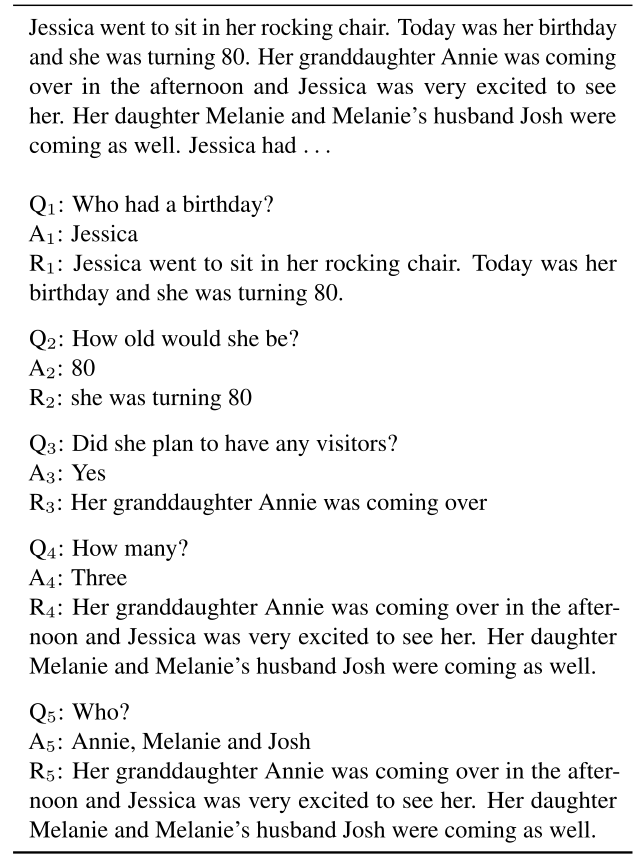
\includegraphics[width=0.5\textwidth]{coqa.png}
%     \end{figurehere}
% \end{center}

\subsection{带有无答案问题的阅读理解}\label{unknown}
早期的MRC数据集全都有一个共同的特点就是默认每一个问题都可以在给定的文本中找到答案,然而一段文本所包含的知识是有限的,因此有下述两点是需要考虑的:(1)这段文本不能回答那些与文本表达内容无关的问题;(2)某些问题可能与文本内容类似但是问题含义与文本含义不同。这两种问题都属于无答案问题,不能从给定的文章中找到问题的答案。
目前流行的带有无答案问题的数据集如SQuAD 2.0\upcite{SQuAD2},在SQuAD的基础上增加了五万多个无答案问题。一个样例如表9所示,文章中Bald Eagle Protection Act指的是1940 treaty的名字,并不是
问题所问的1937 treaty的名字。
\begin{table}[ht]
	\centering
	\caption{SQuAD 2.0的一个样例 \\ Table 9 An example of SQuAD 2.0}
	%\vspace{5pt}
	\begin{tabular}{l p{13.2cm}<{\raggedright}}
		\toprule
		文章:&\tabincell{l}{Other legislation followed, including the Migratory Bird Conversation Act of 1929, \\ 
			a \textbf{1937 treaty} prohibiting the hunting
			of right and gray whales, and the \\ 
			\textbf{Bald Eagle Protection Act of
			1940}. These later laws had a low cost to society\\ —the species
			were relatively rare—and little opposition was raised.}\\
		%\cmidrule(l){2-3}
		\midrule
		问题:&\tabincell{l}{What was the name of the 1937 treaty?} \\
		%\cmidrule(l){2-3}
		\midrule
		看似合理的答案:&Bald Eagle Protection Act \\
		\bottomrule
	\end{tabular}
\end{table}
如果不考虑问题的可答性,仅仅依靠单词相似度匹配的模型很容易给出看似合理的答案。
对于这类任务模型必须区分出哪些问题是无答案的,对于无答案的问题模型不能再给出``貌似合理"的答案。在3.2节所介绍的模型里,很多模型在SQuAD数据集上表现很好然而在SQuAD 2.0数据集上效果显著下降,这说明很多模型只是基于浅层的语义匹配来寻找答案而不是真正的理解了文章的含义。

对于带有无答案问题的阅读理解任务,模型要分为两个模块:(1)答案抽取模块;(2)判别无答案问题模块。
答案抽取模块用来预测出答案在文章中的位置,第三章所介绍的MRC模型大部分都可以作为答案抽取模块,判别无答案问题模块用来判断当前问题是否可以回答。
Clark等人\upcite{Clark}尝试在原有的答案抽取模块的基础上额外添加一个专门用来预测无答案情况的网络层,此时损失函数定义如下:

\begin{equation}
	L_{joint}=-\log(\displaystyle\frac{(1-\delta)e^z+\delta e^{\alpha_a\beta_b}}{e^z+\sum_{i=1}^{l_p}\sum_{j=1}^{l_p}e^{\alpha_i\beta_j}})
\end{equation}
其中$z$表示模型预测该问题是不可回答问题的分数,如果问题是可以回答的那么$\delta=1$,反之$\delta=0$。$\alpha$和$\beta$分别表示输出层预测的文章中每一个单词作为答案起始位置和终止位置的概率,$a$和$b$分别代表标准答案在文章中的起始位置和终止位置。

由公式(17)可以看出预测的答案跨度分数$\alpha_a,\beta_b$和判断无答案问题的分数$z$是共同归一化的。Hu等人\upcite{ReadVerify}认为两个分数共同归一化会出现冲突,如果模型过分信任预测的答案跨度分数那么就会在预测的无答案问题时产生较低的分数。此外之前的模型并没有验证答案抽取模块预测的答案跨度的合理性。
%所在的句子\footnote{原文中称为answer sentence}可以蕴含出这段跨度文本。
为了解决以上问题,他们提出Read+Verify架构。其中Read模块就是指答案抽取模块+判别无答案问题模块,
Verify模块用来进一步验证是否答案抽取模块预测的答案跨度所在的句子(原文中称为answer sentence)就是标准答案所在的句子。
为了解决上面提到的冲突问题,在Read模块中额外增加了两个辅助损失函数:
\begin{gather}
	L_{indep-span}=-\log(\displaystyle\frac{e^{\widetilde{\alpha}_{\widetilde{a}}\widetilde{\beta}_{\widetilde{b}}}}{\sum_{i=1}^{l_p}\sum_{j=1}^{l_p}\widetilde{\alpha}_{i}\widetilde{\beta}_{j}}) \\
	L_{indep-unknown}=-(1-\delta)\log\sigma(z)-\delta\log(1-\delta(z))
\end{gather}
其中$L_{indep-span}$代表答案抽取模块的损失函数,而此时的答案抽取模块是独立的预测答案片段而不考虑问题是否可以回答,$\widetilde{\alpha}_{\widetilde{a}}$和$\widetilde{\beta}_{\widetilde{b}}$表示的就是答案抽取模块所预测出来的答案跨度。
$L_{indep-unknown}$代表判断问题无答案的损失函数,同样它是独立于答案抽取模块的。$\sigma$代表sigmoid函数。
最后整个Read模块的损失函数定义为:
\begin{equation}
	L_{Read}=L_{joint}+\gamma L_{indep-span}+\lambda L_{indep-unknown}
\end{equation}
$\gamma$和$\lambda$是两个超参数。实验表明去掉$L_{indep-unknown}$后模型在判断无答案问题上的准确率显著下降,证明了上述提出的冲突确实存在。对于Verify模块,他们采用三种结构。第一种将预测出来的答案片段连同问题以及answer sentence连接成一个句子送入预训练模型GPT\upcite{GPT}中预测无答案的概率。第二种采用交互式结构,通过注意力机制计算它们之间的关联。第三种结构是前两个结构的结合,具体的就是将前两个结构的输出张量拼接,实验证明这种混合结构使得模型效果更好。关于处理无答案问题阅读理解任务的其它相关模型可以参考\upcite{Levy,UNet}。

%人在做阅读理解问题的时候通常会先带着问题大致的浏览一下这篇文章,对这篇文章的含义有一个大致的了解。之后再根据问题详细的阅读文章寻找答案。受到这种阅读形式的启发,Zhang等人\upcite{Retrospective}提出一种回顾式阅读器(Retrospective Reader,Retro-Reader)模型。整个模型由两个步骤构成:(1)第一步先简要的略读文章,建模文章与问题的大致关联给出初步的判断该问题是否可以回答。(2)第二步是精读模块,目的是验证可回答性并且给出最终判断。模型的编码器采用强大的预训练模型ALBERT,在SQuAD 2.0数据集上显著优于其它模型。



\subsection{多段落阅读理解}
%典型的机器阅读理解任务都是预先给定一篇文章然后给出与文章相关的问题,这并不符合人们现实生活中的问答场景。人们通常是先提出问题然后从一篇或多篇文章中寻找答案
目前大多数的研究热点集中于单段落阅读理解,仅需要从一个段落上寻找答案,这对模型的阅读理解能力要求不高,此外真实场景中人们往往是从多篇段落中寻找与问题相关的答案最后互相比对得出最准确的答案。
多段落阅读理解任务,一个问题$Q$会对应着
多个相关的段落$(D_1,D_2,\cdots,D_K)$,模型需要从这$K$个段落中寻找最佳答案$A$,建模概率
\begin{equation}
	P(A|D_1,D_2,\cdots,D_k,Q) \notag
\end{equation}

多段落阅读理解也可以认为是开放领域(Open-domain)问答的一种形式。Open-domain问答目的是从广泛的领域资源(如维基百科,网页搜索等)寻找问题的答案而不限于仅仅在某段文本中,这更贴近于真实场景但同时具有相当大的难度。Chen等人\upcite{DrQA}提出利用检索+阅读(Retrieve+Read)的模式处理open-domain问答,先利用检索模块(Document Retriever)从维基百科中获取5个与问题最相关的段落,然后利用阅读器(Document Reader)预测出答案所在的位置。其中Document retriever采用基于TF-IDF权重的词袋向量模型,用来比较问题和文章的关联程度并且在此基础上用bigram哈希优化。

%对于open-domain问答任务,检索模块要检索出与问题相关的文章,因此检索模块的性能极大地影响着模型整体的效果。如果简单的增加其检索文章的数量就可能导致有不相关的文章被检索出,仍然影响后续阅读模块。为了解决这个问题,Lee等人\upcite{Ranking}提出段落排序(Paragraph Ranker)机制,目的是从多篇文章中的多个段落选出与问题最相关的几个段落。具体做法就是利用BiLSTM获得每一篇段落和问题的表示向量,然后计算两个向量的内积作为这篇段落与问题的相似度。

目前典型的多段落数据集如MS MARCO\upcite{MSmarco}、TriviaQA\upcite{TriviaQA},中文的有DuReader\upcite{DuReader}。
以MS MARCO数据集为例,数据集样例见表4. MS MARCO由微软亚洲研究院发布,问题和文章来源于
必应搜索,答案由人工生成,因此数据集接近真实应用场景而且答案不在局限于文章中
。每个问题对应10个由必应搜素引擎返回的文本段落,其中包含答案依据用来回答问题的段落用$\text{is\_select=1}$标记为1。

多段落阅读理解的难点在于模型需要阅读多篇文章,更重要的是每篇文章都有可能包含与标准答案类似的句子,而有些是错误的答案,模型需要排除众多的干扰项选择最正确的答案。想要达到这个目的,要求模型能够解决跨段落实体消歧和跨段落答案验证等问题。

Tan等人\upcite{SNet}提出S-Net模型,
先通过片段抽取模块提取出
一段文本作为答案的预测依据,然后利用生成模块生成答案。其中片段抽取模块采用多任务学习策略,
除了预测文本片段之外还添加一个段落排名任务,
将标记为$\text{is\_select=1}$的段落视为正例。答案生成模块采用seq2seq模型,
其中encoder端的输入是问题和文章的向量表示,同时将片段抽取模块的输出作为额外的特征
拼接到文章中。实验证明S-Net在MS MSRCO数据集上的效果要显著地优于
R-Net\upcite{RNet},ReasoNet\upcite{Reasonet}这些单独做片段抽取任务的模型。

由于不同的段落都有可能包含与标准答案类似的句子,但是有些答案并不是正确的。基于这个问题,Wang等人\upcite{VNet}提出一种模型使得来自不同段落的候选答案在基于它们所在的上下文内容里互相验证对方的正确性。具体的就是将每一篇段落中预测出来的答案与其它段落预测的答案做交互验证。这样做的原因是经观察发现,相比于错误的答案正确答案中的单词往往会在多个段落中重复出现,因此通过交互验证可以凸显出正确答案。最后模型在MS MARCO数据集上的效果优于S-Net。
关于解决多段落阅读理解问题的相关工作可以参考\upcite{zhuang,HuMulti,WangMulti}。

\subsection{对话型阅读理解}\label{cmrc}
%虽然本节介绍的对话型任务按照答案形式上划分仍然可以划分到那四种类型里面,但是由于对话型问答任务与其它任务在数据集构造方式以及任务形式上有较大不同,因此本节单独列出对话型问答任务。
%除了按照答案形式上划分还可以根据文章类型划分,如单段落型阅读理解还是多段落型阅读理解。
%
%
%根据问答形式划分,比如上面所介绍的所有数据集都属于单轮对话式问答,
%即文章所对应的多个问题之间没有联系,每一个问题都是互相独立的。这并不符合
%现实世界中人与人之间的对话交流,人们是通过多轮对话形式来交流的,每一轮的问题和答案都会影响后面的问答情况。
无论是单段落阅读理解还是多段落阅读理解任务,它们都属于单轮对话问答,即问答的形式只有一轮,后面的问题与前面的问题和答案无关,每一个问题都是互相独立的。
而在真实场景中人们是通过多轮对话形式来交流的,每一轮的问题和答案都是基于前面的问答情况。
所以针对对话型阅读理解问题,在回答当前轮的问题时不仅需要考虑文章还需要考虑前几轮的问题和答案。
具体可以表示为:给定$Q_i,D,Q_{i-1},\cdots,Q_{i-k}$以及$A_{i-1},\cdots,A_{i-k}$要求模型给出$A_{i}$。其中$Q_i,A_i$表示第$i$轮的问题和答案,$D$表示文章,$Q_{i-1},\cdots,Q_{i-k}$和$A_{i-1},\cdots,A_{i-k}$分别表示前$k$轮的问题和答案。即建模概率:
\begin{equation}
P(A_i|D,Q_i,Q_{i-1},\cdots,Q_{i-k},A_{i-1},\cdots,A_{i-k})
\end{equation}

目前典型的对话型阅读理解数据集有CoQA\upcite{CoQA}以及QuAC\upcite{QuAC}。
不同之处在于CoQA数据集的答案形式较为简单,类似于SQuAD\upcite{SQuAD1},但是包含有yes/no以及无答案问题,此外还有一定比例的问题是自由答案形式。
%QuAC数据集的答案全部是抽取式的。
%而QuAC数据集的构造过程中提问者没有看过文章而仅仅了解文章的标题,由回答者根据文章的内容选择出文章的一段文本作为答案,这种数据集构造形式类似于用户在搜素引擎中输入问题查找答案,目的是减少问题和文本之间的依赖,使得模型尽量避免通过浅层的匹配方式获得答案。
对话型阅读理解数据集的一个样例见表10。

\begin{table}[ht]
	\centering
	\caption{CoQA\upcite{CoQA}数据集的一个样例 \\ Table 10 An example of CoQA}
	%\vspace{10pt}
	\resizebox{\textwidth}{!}{\begin{tabular}{l p{15.5cm}<{\raggedright}}
			\toprule
			\multirow{3}{*}{文章}&Jessica went to sit in her rocking chair. Today was her birthday and she was turning 80. Her granddaughter Annie was coming over in the afternoon and Jessica was very excited to see her. Her daughter Melanie and Melanie's husband Josh were coming as well.\\
			\cmidrule{2-2}
			\multirow{3}{*}{第一轮}&$Q_1$: Who had a birthday? \\
			&$A_1$: Jessica \\
			&$R_1$: Jessica went to sit in her rocking chair. Today was her birthday and she was turning 80. \\
			\cmidrule{2-2}
			\multirow{3}{*}{第二轮}&$Q_2$: How old would \textbf{she} be? \\
			&$A_2$: 80 \\
			&$R_2$: she was turning 80. \\
			\cmidrule{2-2}
			\multirow{3}{*}{第三轮}&$Q_3$: Did \textbf{she} plan to have any \textbf{visitors}? \\
			&$A_3$: Yes \\
			&$R_3$: Her granddaughter Annie was coming over \\
			\cmidrule{2-2}
			\multirow{3}{*}{第四轮}&$Q_4$: \textbf{How many?} \\
			&$A_4$: Three \\
			&$R_4$: Her granddaughter Annie was coming over in the afternoon and Jessica was very excited to see her. Her daughter Melanie and Melanie's husband Josh were coming as well. \\
			\cmidrule{2-2}
			\multirow{3}{*}{第五轮}&$Q_5$: \textbf{Who?} \\
			&$A_5$: Annie, Melanie and Josh \\
			&$R_5$: Her granddaughter Annie was coming over in the afternoon and Jessica was very excited to see her. Her daughter Melanie and Melanie's husband Josh were coming as well. \\
			\toprule  
	\end{tabular}}
\end{table}

% \begin{center}
% \begin{figurehere}
%     \textbf{图1:CoQA\upcite{CoQA}数据集的一个样例}
%     \vspace{10pt}
%     \centering
%     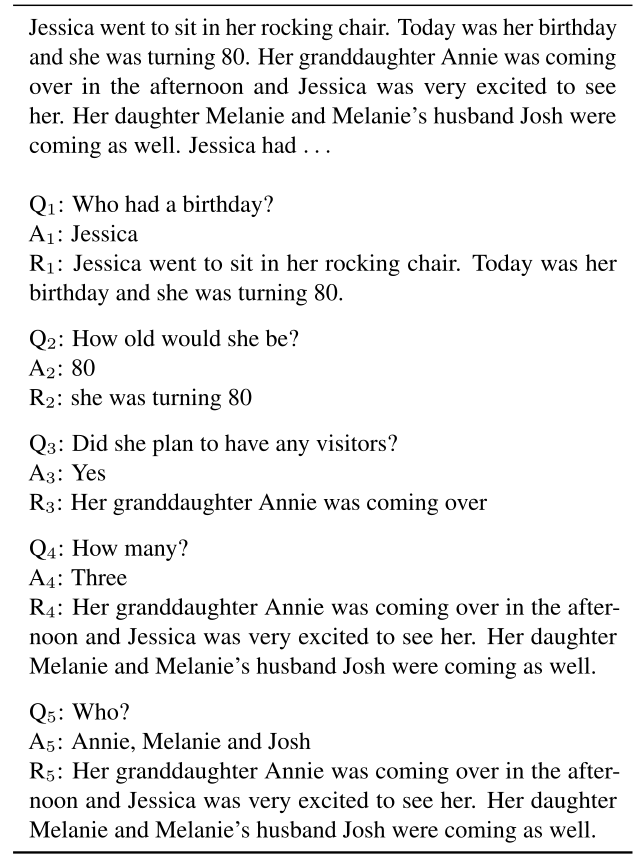
\includegraphics[width=0.5\textwidth]{coqa.png}
% \end{figurehere}
% \end{center}
其中每一个$Q_i$和$A_i$代表问题和对应的答案,每一个$R_i$表示给出这个答案的依据,用来训练模型。
测试集中是没有答案依据的。
%因此对话型问答任务可以描述为给定文章$P$和
%历史的对话信息$Q_1,A_1,Q_2,A_2,\cdots,Q_{k-1},A_{k-1}$,任务的目的是
%给出第$k$轮的问题$Q_k$的答案$A_k$。
从图中可以清楚地看到$Q_2$和$Q_3$中的she指代的是$Q_1$的答案$A_1$,而$Q_4$的How many?以及$Q_5$的Who?所问的
是$Q_3$中的visitors。显然单独靠当前轮的问题是无法回答的,对于这类任务模型必须解决指代消解问题以及
如何利用对话历史信息。

Reddy等人\upcite{CoQA}
%采用三种模型在CoQA数据集上进行实验。
%第一种是传统的seq2seq模型,decoder用来生成答案。第二种是指针生成网络(Pointer-Generator Network\upcite{PGNet},PGNet),既可以从词典中生成答案又可以从原文中拷贝单词,很好的解决了OOV(Out Of Vocabulary)问题。
%第三种是DrQA+PGNet模型,其中DrQA\upcite{DrQA}是一个片段抽取模块。整个模型的思想是
%先利用片段提取模块从文章中提取中与问题最相关的一段文本,然后利用答案生成模块在这个被抽取出来的文本上
%生成答案。这种(提取模块+生成模块)模型在其它的生成模型中如S-Net\upcite{SNet}等广泛使用。
%实验结果也表明这种模型的效果是最好的。
首先提出将前几轮的问题与答案结合到
段落中,从而能够利用历史的对话信息回答当前轮的问题。
%\begin{center}
%    \begin{figurehere}
%        \textbf{图2:CoQA\upcite{CoQA}数据集的一个样例}
%        \vspace{10pt}
%        \centering
%        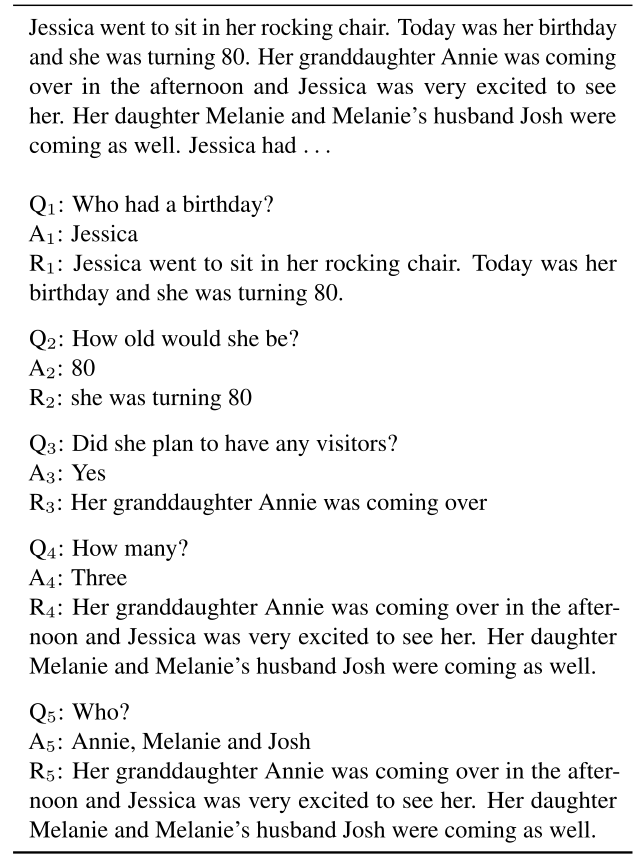
\includegraphics[width=0.5\textwidth]{coqa.png}
%    \end{figurehere}
%\end{center}
Choi等人\upcite{QuAC}利用BiDAF++\upcite{Clark}模型在QuAC数据集上进行实验,为了利用历史的对话信息,在文章中设置一个标记向量用来标记段落中的单词是否是历史答案,将问题的轮次作为额外特征添加在问题向量上。
%Yatskar等人\upcite{CompareSQC}采用同样的模型以及同样的历史信息处理方式在CoQA数据集上进行实验,由于CoQA数据集包含有yes/no问题,因此在输出层额外设计预测yes/no的情况。

Huang等人\upcite{FlowQA}认为上述的方法只是简单的添加之前轮的问题和答案,而忽略了在回答之前轮问题时模型对整篇文章的推理过程状态。因此他们提出一种带有流机制的模型FlowQA,目的是将模型处理每一轮的问答过程下的对文章的语义理解状态流向下一轮的问答过程。FlowQA模型整体上利用双向循环神经网络编码文章,利用单向循环神经网络编码对话历史,对比之前的模型,FlowQA能够集成更加深层次的对话历史状态。

%虽然预训练模型BERT\upcite{BERT}在自然语言理解任务上展现出其强大的性能,但是其数据输入形式只能是两个句子的拼接因此并不适合直接处理对话型任务。Qu等人\upcite{HAE}提出一种简单而有效的模型,仅仅需要在BERT模型的输入端为每一个单词添加两个额外的向量用来表明这个单词有没有在历史答案中出现过,文中称这两个向量为(History Answer Embedding,HAE)。实验表明BERT+HAE模型较之前的模型可以处理更多的历史对话信息。
%Zhu等人\upcite{SDNet}
%提出的SDNet模型,以基于特征的方式迁移BERT作为编码器,同时将之前轮次的问题和答案拼接到当前轮的问题上构成一个新问题。模型采用自注意力机制获得历史对话信息之间的交互语义,具体的计算方式采用FusionNet\upcite{Fusionnet}模型提出的融合方法。
%Ohsugi等人\upcite{simpleqa}以基于微调的方式迁移BERT模型。
%将历史对话信息每一轮的问题与答案分别与文章连接送入
%BERT,将每一个BERT的输出连接作为输出层的输入。





值得注意的是尽管CoQA数据集有部分答案是自由答案形式的,但是上面的模型大多是利用片段抽取式的做法在CoQA数据集上实验,主要原因在于
生成式模型的效果往往不如抽取式模型的效果好,因为生成式模型对答案生成模块要求较高。
因此如何提高模型的答案生成能力是值得进一步研究的方向。
由于预训练模型UNILM\upcite{UNILM}改进了BERT的训练任务,
增加了自回归语言模型以及seq2seq语言模型使得其
在生成式任务上的效果很好,在CoQA数据集上远远的超过于Reddy等\upcite{CoQA}提出的生成式基准模型。关于如何迁移预训练模型在对话型阅读理解任务上的相关工作可以参考\upcite{HAE,SDNet,simpleqa}。

%\subsection{小结}
%本章介绍了MRC领域目前较为复杂的任务:带有不可回答问题的任务,多段落型任务以及对话型问答任务。相比于之前介绍的阅读理解任务,这三个任务都有各自的特点和难点所在。实验表明之前的经典模型在比较简单的数据集上已经达到了很好的效果,然而迁移到这几个复杂的阅读理解任务上模型效果显著下降。如何设计性能更加强大的模型来处理更加复杂的任务还需要大量的研究。




